\section{Results}

All results describing the correctness of the simulation or discussing the closeness of the simulation to an analytical
result are done using the single-threaded mode. This is because this makes the result of the simulation deterministic,
and so it does not matter which machine the test was run on. For results that measure performance, the machine and options
for the simulation used will be specified. There are times when the number of threads affected the correctness of the
result.

Additionally, all results presented use the successive over-relaxation method for calculating the solution. This is because
it converges more quickly on a solution that Jacobi iteration. Both methods produce the same results (as long as the Jacobi
iteration runs for long enough), so the correctness results are unaffected by the choice of algorithm. Secondly, the performance
measurements measure iterations per second, which is also largely independent of the choice of algorithm. Since successive
over-relaxation is so much more effective at quickly converging upon a solution, it is presented as the program's primary
mode of operation, with Jacobi iteration provided as a secondary and deprecated option.

\subsection{The $\sin(x)$ Potential}

	\begin{figure}[h!]
	\centering
	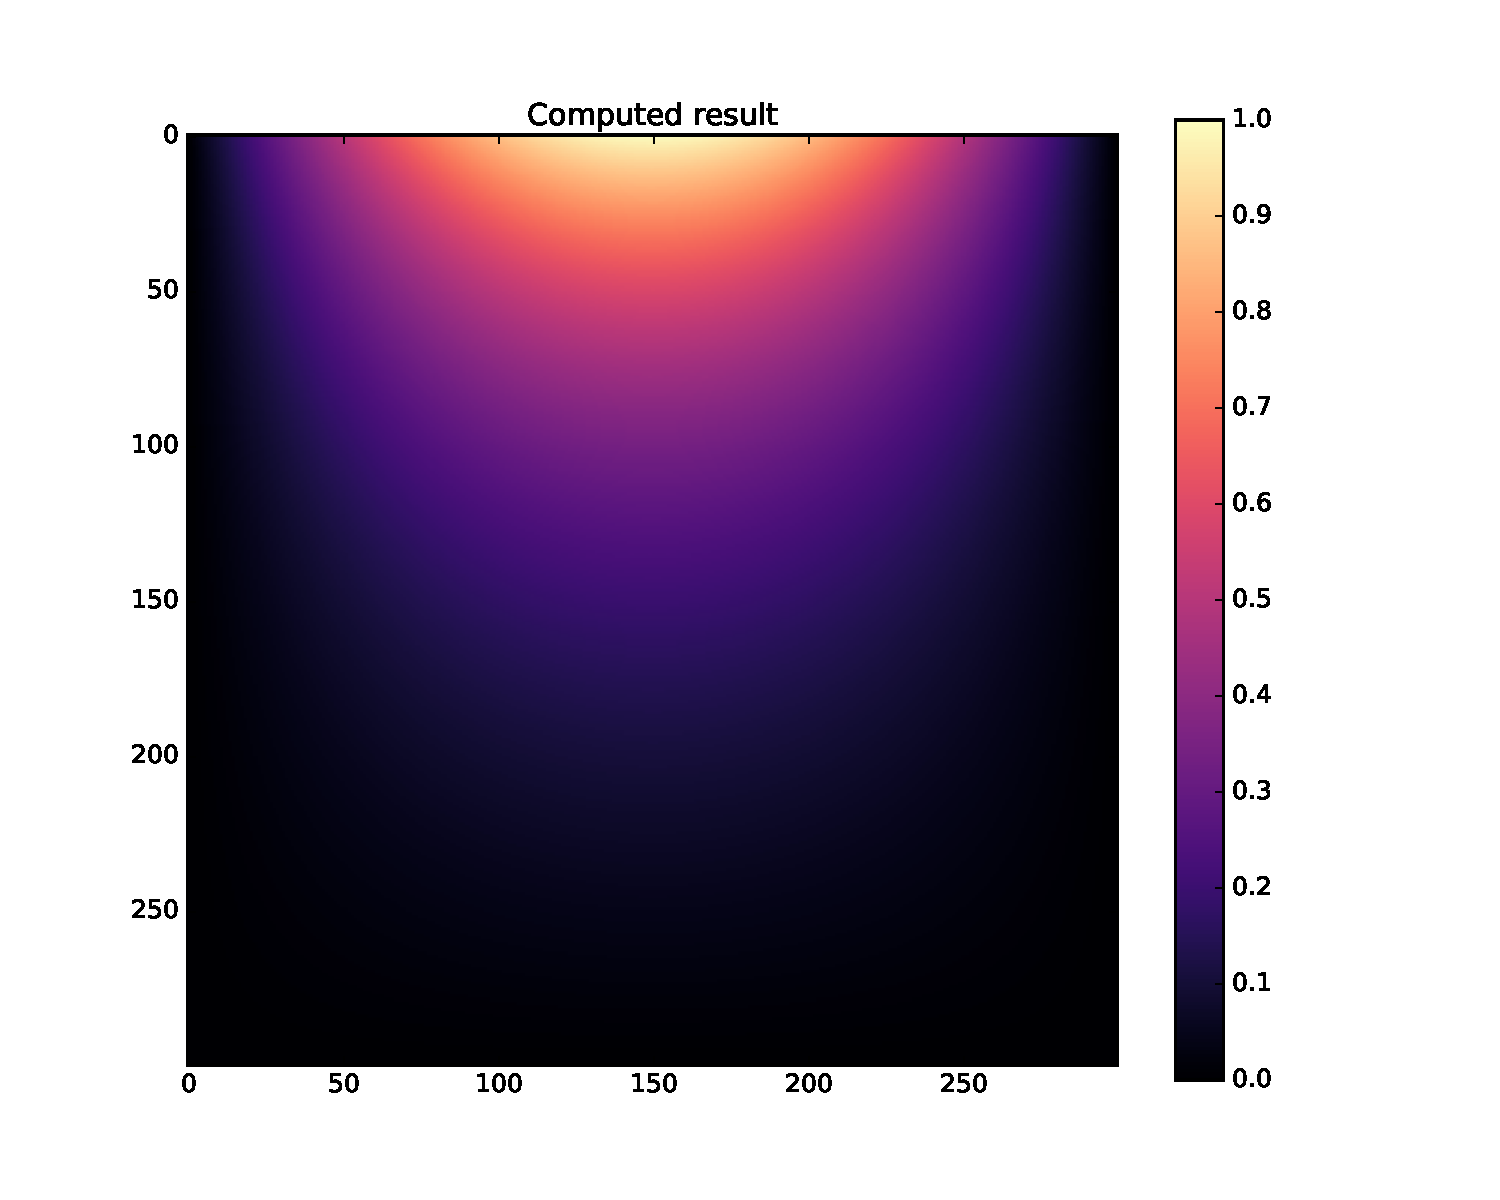
\includegraphics[width=1.1\linewidth]{sin300_calc.pdf}
	\caption{Result of simulation for the $\sin(x)$ potential, computed on a 300 by 300 grid.} 
	\label{fig:sin-result}
	\end{figure}

\begin{figure}[h!]
	\centering
	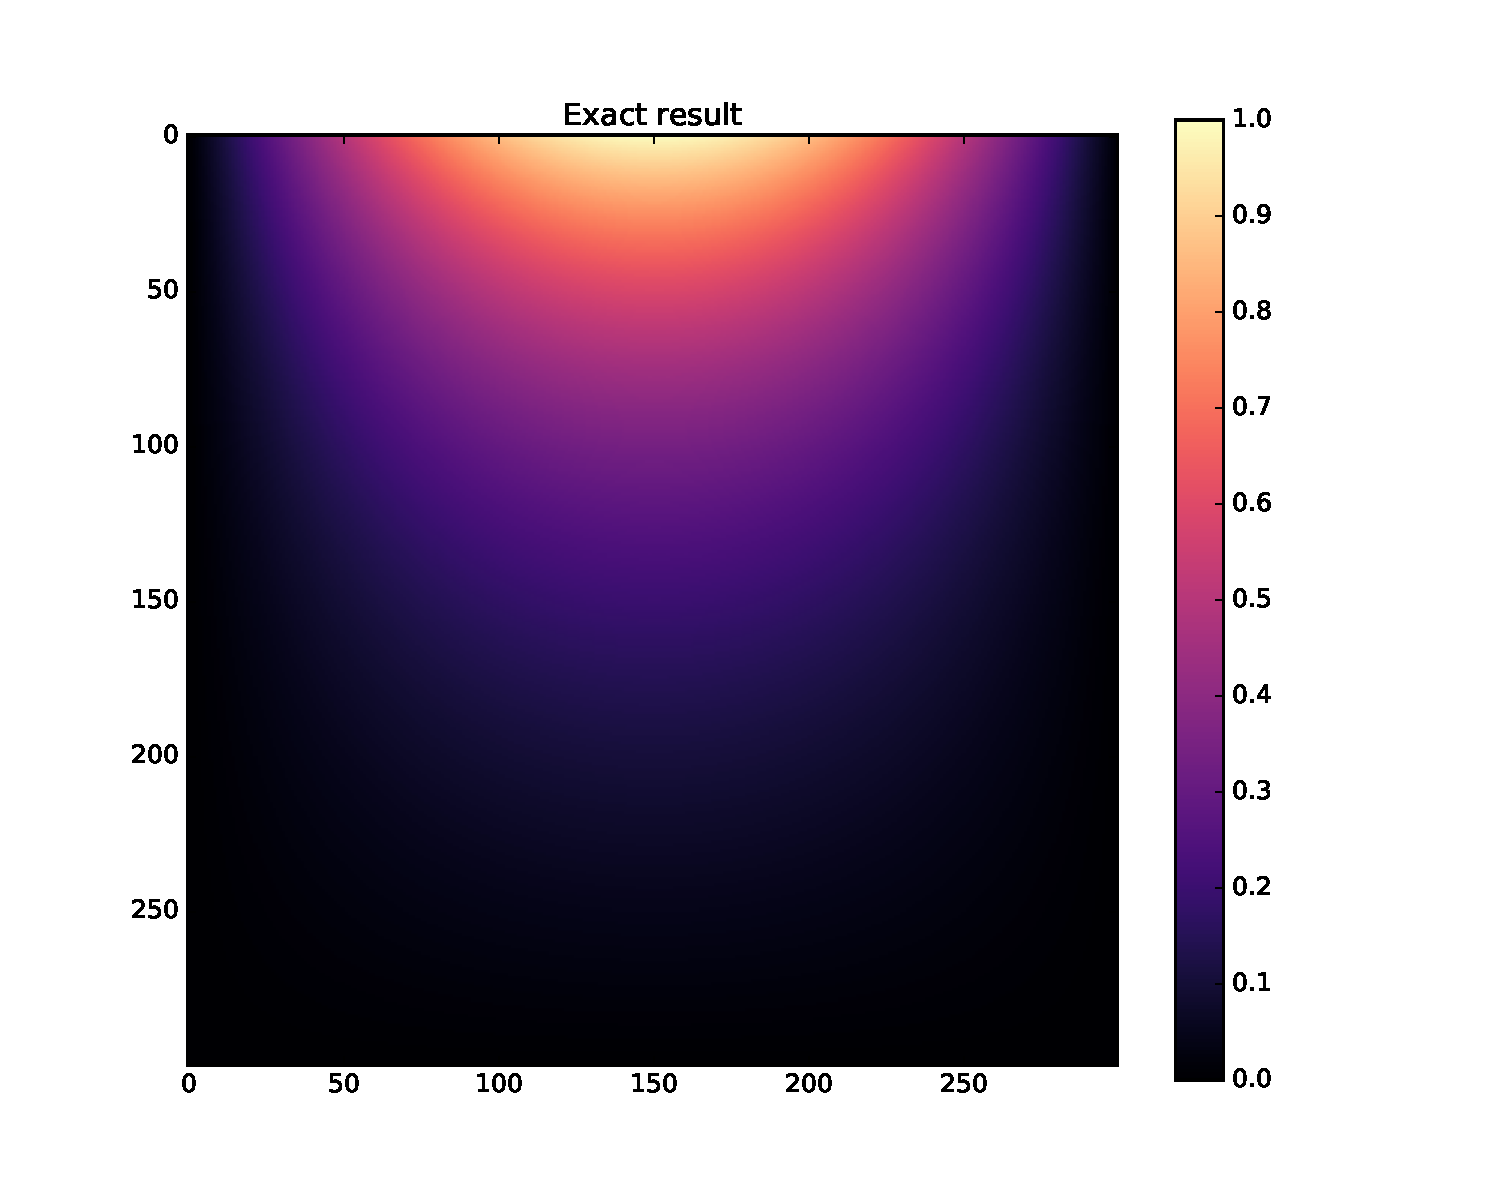
\includegraphics[width=1.1\linewidth]{sin300_exact.pdf}
	\caption{Analytical result for the $\sin(x)$ potential, with the same initial conditions and boundary conditions as the simulation.}
	\label{fig:sin-analytic}
	\end{figure}



Figure~\ref{fig:sin-result} shows the output of the solver program in single-threaded mode when given the $\sin(x)$ along one side
potential, plotted with the Python library matplotlib. The configuration has a grid size of 300 by 300. It matches well with the analytical result, which
is
$$\frac{\sinh(y \pi / n)}{\sinh(\pi)} \sin(x \pi / n),$$
and is shown in Figure~\ref{fig:sin-analytic}. The difference between the calculated result and the
analytical result is shown in Figure~\ref{fig:sin-difference}. The values shown in the difference map are small compared
to the values in the result in all locations except the corners at the top, where the simulation does diverge somewhat, 
but never reaches values which are hugely divergent from the analytical result. Using the root-mean-square error statistic
described earlier, we have calculated the RMS error in this simulation to be 0.0025. The mean of all the cell values in this
simulation is 0.19, so the mean error per cell is 1.3\%. The error is small compared to the mean value of all of the cells,
showing that the simulation result is of high quality.


	\begin{figure}[h]
	\centering
	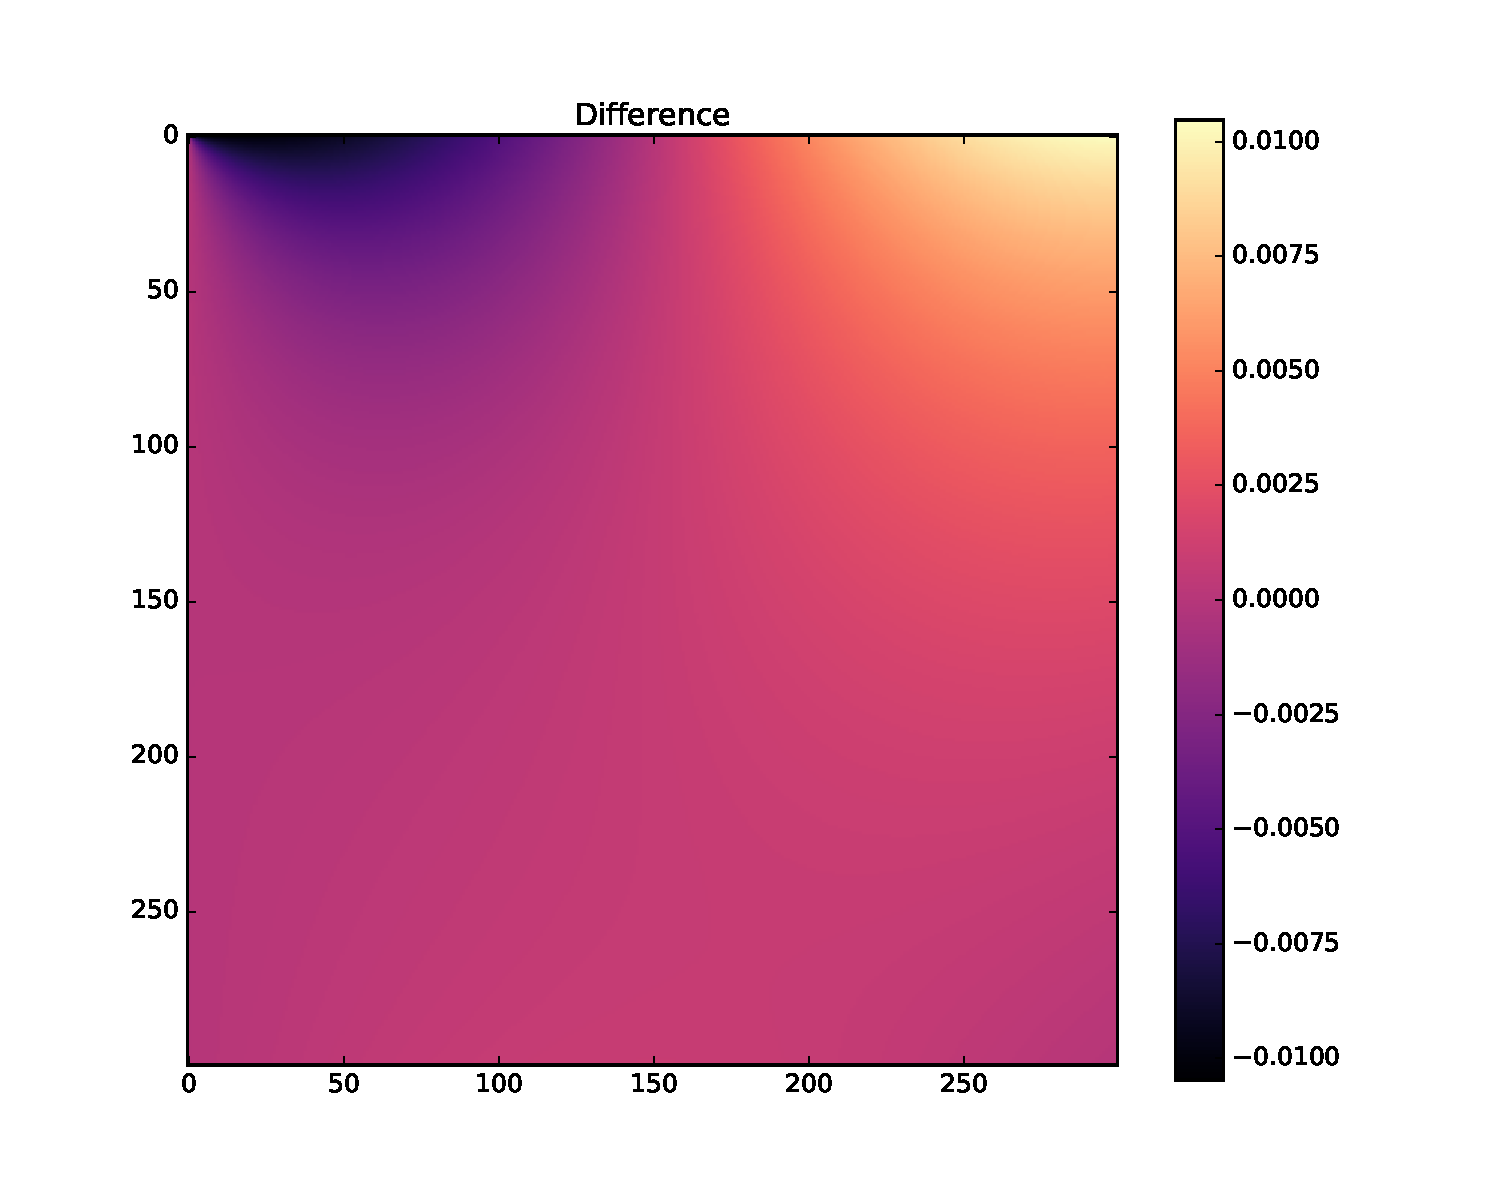
\includegraphics[width=1.1\linewidth]{sin300_diff.pdf}
	\caption{Difference between the calculated and analytical results for the $\sin(x)$ potential.}
	\label{fig:sin-difference}
	\end{figure}

\subsection{Fitting to a $1/r^2$ Dipole Potential}
\begin{figure}[h!]
	\centering
	\center
	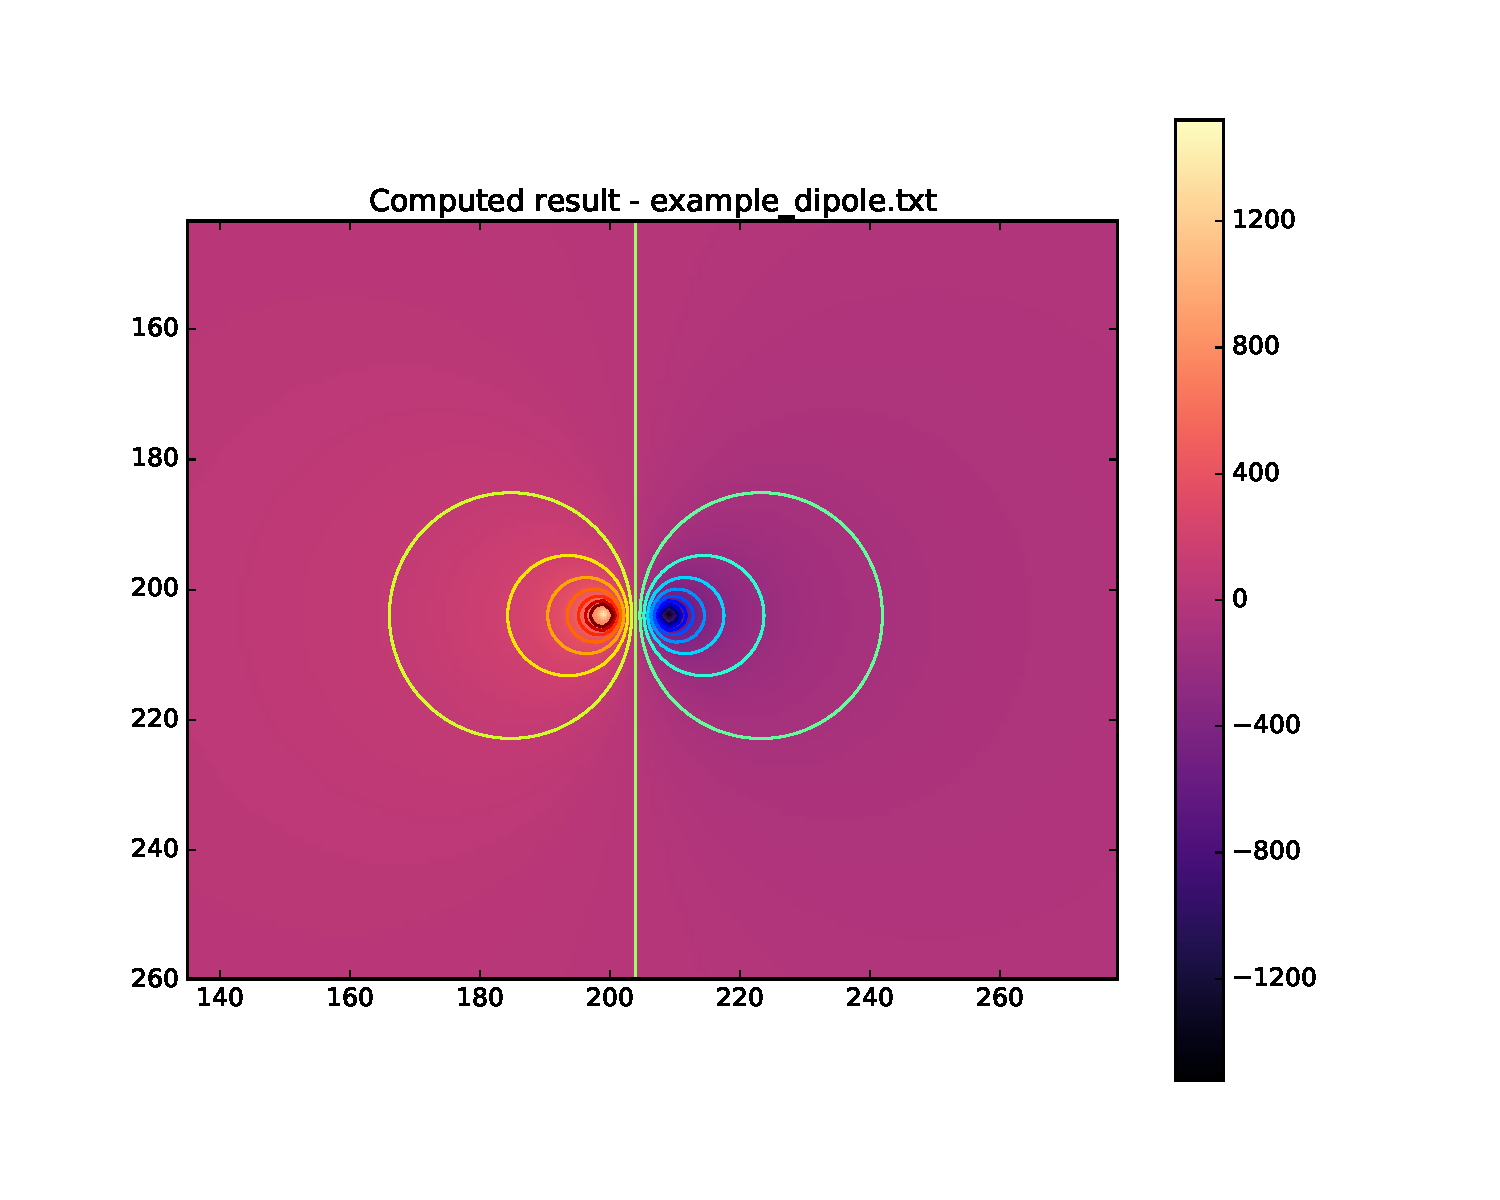
\includegraphics[width=1.0\linewidth]{dipole_contours.pdf}
	\caption[Result of the simulation for the dipole configuration, including contour lines.]{Result of the simulation for the dipole configuration, including contour lines. The vertical line in the center shows that there is a line of constant, zero-valued
	potential at points equidistant from the two charges, which is what one would except to see from a dipole. Note that this is zoomed in on the result, as otherwise the features
	would be too small.} \label{fig:dipole-cont}
	\end{figure}


The dipole configuration had a grid size of 400 by 400, with all walls given a Dirichlet boundary condition
of zero. Two charges were placed near the center 10 cells apart with an arbitrary but equal and opposite charge.
The result of this simulation is shown in Figure~\ref{fig:dipole-cont}, with the addition of constant-potential
contour lines. The simulation shows two opposite charges which near perfectly mirror each other. The vertical
line in the center represents a constant potential contour with a value of zero, which is expected from an
electric dipole. This is another excellent verifier that the simulation is producing correct results.

	\begin{figure}[h!]
		\centering
	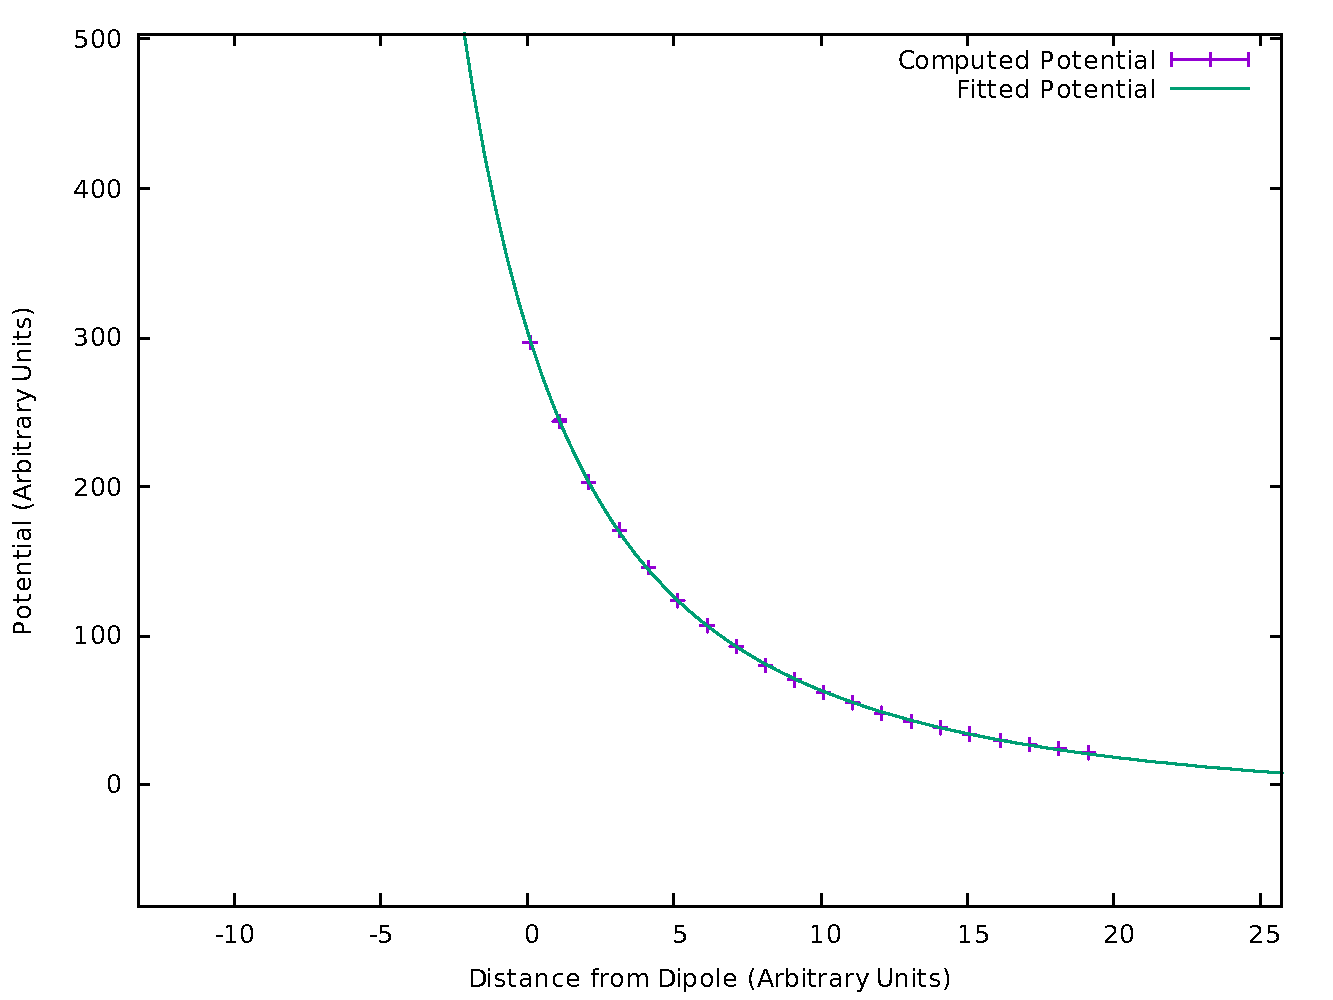
\includegraphics[width=\linewidth]{dipole_fit.pdf}
		\caption[Fitting a $1/r^2$ curve to the calculated dipole potential.]{Fitting a $1/r^2$ curve to the calculated dipole potential. Both the units of the distance and the value of the potential are taken into account in the fitting by providing
		the necessary constants for the fit. The error bars are from the RMS error per cell as described earlier.} \label{fig:dipole-fit}
	\end{figure}



I then measured the potential at locations increasing in distance from the dipole in an arbitrary direction.
These data were then plotted using gnuplot, and a line of the form $y(x) = A + B / (r-r_0)^2$ was fit to the
data, which is shown in Figure~\ref{fig:dipole-fit}. The fit is excellent, confirming that the program had properly simulated an electric dipole.

The dipole is an example which lends itself to presenting another feature of the solver program. If passed the
$\texttt{-V}$ option, it will take the negative gradient of the result and plot that as a vector field. This has
the effect of plotting the electric field of the result of the simulation, which for the dipole is shown in
Figure~\ref{fig:dipole-field}.

	\begin{figure}[h]
	\centering
	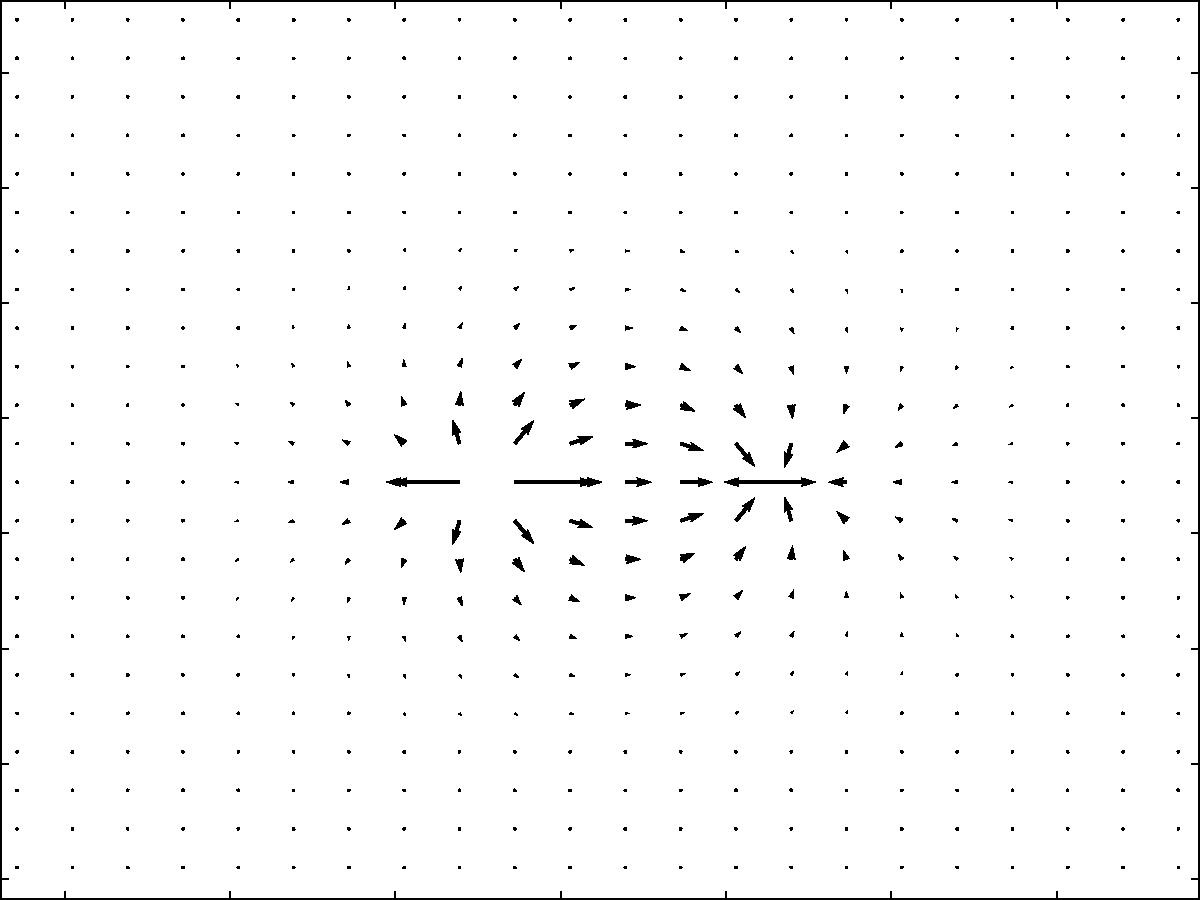
\includegraphics[width=0.7\linewidth]{dipole_field.pdf}
		\caption[Result of program outputting the electric field for the dipole configuration.]{Result of program outputting the electric field for the dipole configuration. At the point of the negative charge,
		the field lines appear to be point outward. They are actually pointing inward but are long enough that they cross each other to form this illusion.} \label{fig:dipole-field}
	\end{figure}


\subsection{Jacobi Iteration Versus Successive Over-Relaxation}
	\begin{figure}[h!]
	\centering
	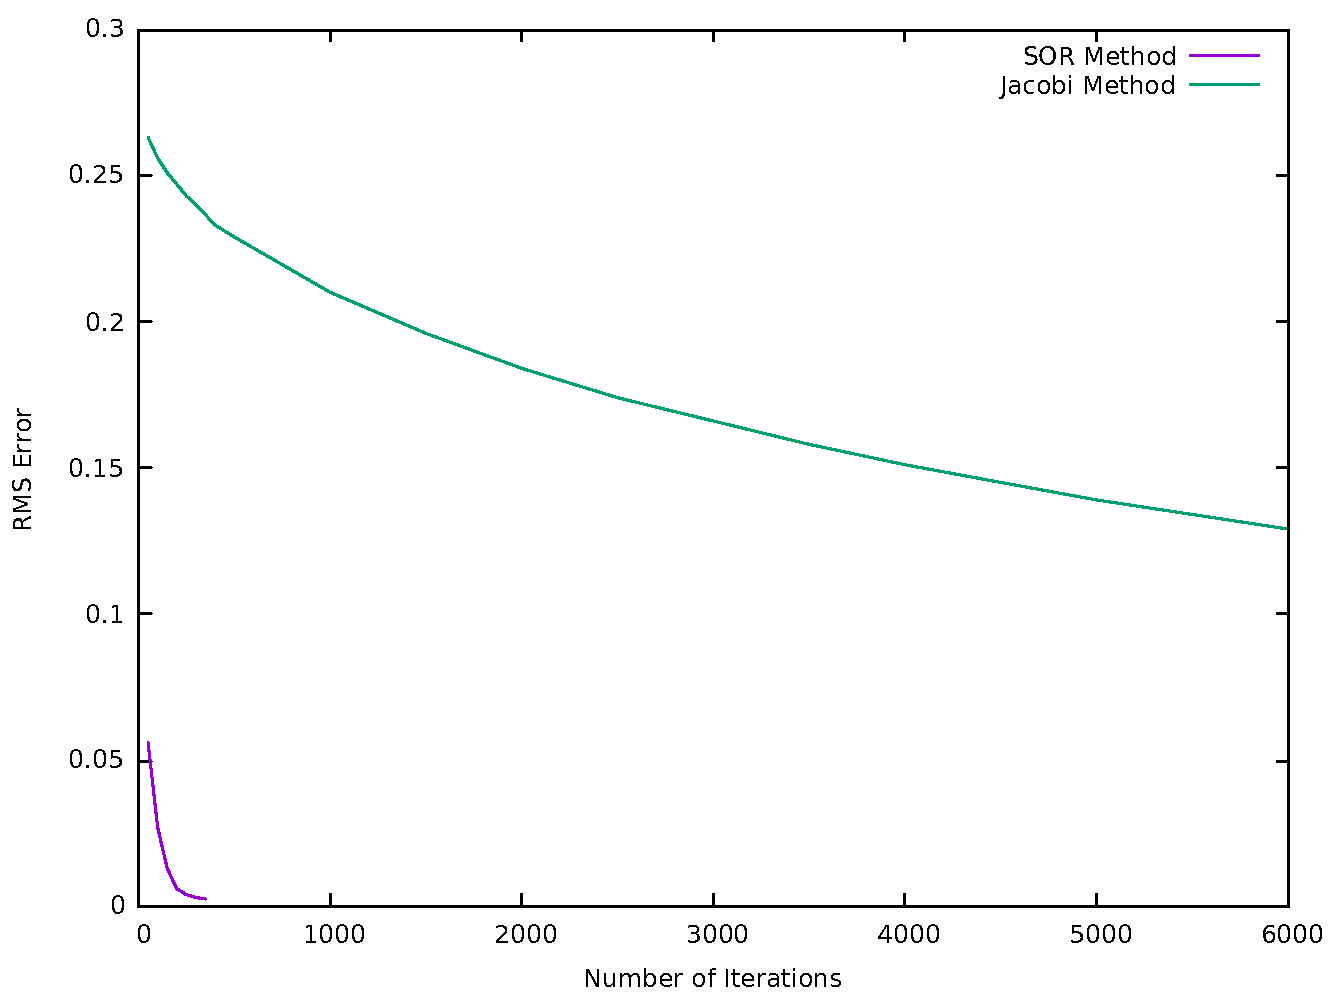
\includegraphics[width=1.0\linewidth]{jacsor.pdf}
		\caption[Convergence of Jacobi iteration and SOR.]{Convergence of Jacobi iteration and SOR. The SOR line is truncated once it reaches convergence. The measurements were made in increments of 50 iterations starting at
		50 until 500, at which point the steps were done in increments of 500. The graphs do not start at zero because the error would be very large and would not assist in
		illustrating the difference between the two methods.} \label{fig:jacsor}
	\end{figure}



Figure~\ref{fig:jacsor} shows the convergence rates for Jacobi iteration and successive over-relaxation. The SOR method
reached convergence rapidly compared to Jacobi iteration -- around iteration 350, whereas Jacobi iteration at the
same iteration was 100 times worse than SOR. This is the reason why I use SOR in most of my analysis; it reaches convergence
so much faster that even if Jacobi iteration were capable of performing twice as many iterations per second, successive over-relaxation
would \textit{still} be much faster to find the solution. This is the power of the asymptotic behavior analysis of different algorithms.


\subsection{Performance}


Figure~\ref{fig:perf-sizes} shows the performance in iterations per second for a varying grid size for a given
configuration, in this case the $\sin(x)$ along a wall potential. The performance tests were run using square grids
of size 50 by 50, 300 by 300, and 1000 by 1000. For each grid size, 4 different simulation options were given:
single-threaded non-SIMD, single-threaded SIMD, multi-threaded with 4 threads non-SIMD, and multi-threaded
with 4 threads SIMD.

\pgfplotsset{compat = 1.3}
\begin{figure}[h]
	\centering
	\pgfplotstableread{
		0 55642.1 3747.52    54100.9 3401     53724.2 13306.44    44877.5 9672
		1 1504 30.6    1461 15     3119 269    2333 313
		2 132.845 1.36    127.085 3.45     297.9 23.13    222.8 26.7
	}\dataset
	\begin{tikzpicture}
    \begin{axis}[
    	xticklabels = {
    		sin50,
    	    sin300,
    	    sin1000,
    	},
        xtick=data,
        ymode=log,
            log ticks with fixed point,
        major x tick style = transparent,
        width  = 0.85*\textwidth,
        height = 8cm,
        major x tick style = transparent,
        enlarge x limits=0.25,
        ybar=2*\pgflinewidth,
        bar width=14pt,
        ymajorgrids = true,
        ylabel = {Run time speed (iters/sec)},
        xtick = data,
        major x tick style = {opacity=0},
        minor x tick num = 1,
        minor tick length=2ex,
        ymin=0,
        legend cell align=left,
		legend style={
	        anchor=south east,
	        column sep=1ex
	    },
        ]

\addplot+[error bars/.cd, y dir=both, y explicit] table[x index=0,y index=1, y error index=2] \dataset; %Data1
\addplot+[error bars/.cd, y dir=both, y explicit] table[x index=0,y index=3, y error index=4] \dataset; %Data2
\addplot+[error bars/.cd, y dir=both, y explicit] table[x index=0,y index=5, y error index=6] \dataset; %Data3
\addplot+[error bars/.cd, y dir=both, y explicit] table[x index=0,y index=7, y error index=8] \dataset; %Data3

	\legend{Single-Threaded SIMD, Single-Threaded, Multi-threaded (4 threads), Multi-threaded (4 threads) SIMD}
\end{axis}
\end{tikzpicture}
	\caption[Performance characteristics for different grid sizes and varying options.]{Different grid sizes for the $\sin(x)$ configuration, and their performance characteristics with different options for the solver. The performance
	also decreases rapidly as the grid size increases.}
\label{fig:perf-sizes}
\end{figure}

In the case of the 50 by 50 grid, the performance was similar for all cases
except for multi-threaded with SIMD. I believe the reason that the SIMD multi-threaded version was slower was
due to the manual SIMD code being less cache-friendly, resulting in the threaded versions having more contention.
Both the 300 by 300 case and 1000 by 1000 case display similar performance behavior: the SIMD case is faster than
the non-SIMD case when single-threaded, and the SIMD case is slower than the non-SIMD case when multi-threaded.
This can be explained in the same way as it was for the 50 by 50 case. Another characteristic is that the multi-threaded
case (with 4 threads) is faster than the single-threaded case. In fact, it is significantly faster than I expected it to be.

Additionally, the performance depends heavily on the grid size. This makes sense, as the amount of work needed to be
done per iteration is proportional to the number of cells in the grid, and the number of cells in the grid is $n^2$.
Another note is that the variance on the performance is significantly higher for all of the multi-threaded cases.
This is because having multiple threads increases the program's dependence on the scheduling quirks of the operating
system. Finally, the variance for the 50 by 50 case multi-threaded versions are significantly higher than all other
variances for the other multi-threaded cases. I believe that this is because the overhead of managing threads compared
to how much work they actually have to do is large in this case compared to the other cases.

\vspace{5mm}

\begin{figure}[h]
	\centering
	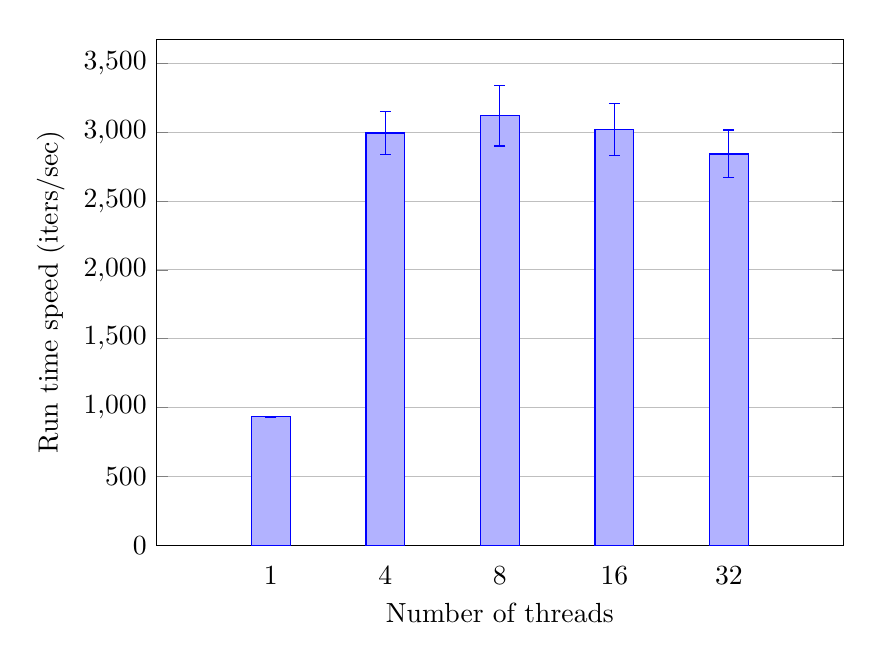
\begin{tikzpicture}
    \begin{axis}[
        xtick=data,
        symbolic x coords={1, 4, 8, 16, 32},
        major x tick style = transparent,
        width  = 0.85*\textwidth,
        height = 8cm,
        major x tick style = transparent,
        ybar=2*\pgflinewidth,
        bar width=14pt,
        ymajorgrids = true,
        ylabel = {Run time speed (iters/sec)},
        xlabel = {Number of threads},
        xtick = data,
        scaled y ticks = false,
        enlarge x limits=0.25,
        ymin=0,
        legend cell align=left,
		legend style={
	        anchor=south east,
	        column sep=1ex
	    },
        ]
            \addplot+[error bars/.cd,
                       y dir=both, y explicit]
                    coordinates {
                    (1, 933.156)  +- (3.612, 3.612)
                    (4, 2994.42)  +- (157.1, 157.1)
                    (8, 3119.1)  +- (219, 219)
                    (16, 3020.6)  +- (190, 190)
                    (32, 2842)  +- (174, 174)
                    };
\end{axis}
\end{tikzpicture}
	\caption[Performance results for varying number of threads.]{Performance results for a varying number of threads in non-SIMD mode. These
tests were done on computer B, using the $\sin(x)$ potential with a grid size of 300 by 300. The performance increases until it reaches a maximum and then degrades after that.}
\label{fig:perf-numthreads}
\end{figure}

Figure~\ref{fig:perf-numthreads} shows the performance in iterations per second of the solver when run
with the $\sin(x)$ potential with a grid size of 300 by 300 with a varying number of threads. This was done on computer B, and so was done
only in non-SIMD mode. The results show a significant improvement in performance when using multiple threads
compared to the single-threaded case. One may na\"{i}vely have expected the performance to scale linearly
with the number of threads; however, this would be unlikely. As the number of threads goes up, the amount
of work that can be done in parallel would seem to scale with the number of threads, until one considers processor cache effects (specifically
cache coherency and cache size limitations). This is seen in the case of 4 threads, as it is not 4 times as fast as
the single-threaded case, only about 3.2 times as fast. Increasing the number of threads quickly starts giving diminishing
returns, as the 8 threads case is now only slightly better than the 4 threads case. Recall that computer B, on which these
tests are run, has 4 cores with 2 threads each, totaling 8 possible threads running in parallel. After the 8 threads case,
we start to see a drop in performance; the 16 and 32 threads case are worse than the 8 threads case. This is because
the machine cannot run more than 8 threads in parallel, so in order to have 16 threads it must rely on the scheduling
of the operating system in order to get work done. In a case of many threads, each doing heavy computation and memory accesses
(as is the case here), it does not usually help to increase the number of threads beyond what the machine can handle,
as is shown here.



Furthermore, Figure~\ref{fig:err-numthreads} shows that it is disadvantageous to run the simulation with
a large number of threads. The RMS error of the simulation compared to the analytical result increases
rapidly with the number of threads. This is also reflected visually in the plotted result of the simulation, which is
noticeably wrong in the case of 16 or higher threads. I believe this is the result of the way the threads
are synchronized, or more accurately, how they are not. The threads run mostly in isolation, sharing the
grid and doing operations on it without waiting for other threads to complete any of their work. This means
that if one threads runs faster than the others, it may complete a different number of iterations than the other
threads in a given amount of time. This would result in some sections of the grid receiving more iterations
than others, which could have the effect of invalidating the simulation. The alternative method would be
to synchronize the threads, and have them wait for each thread to complete a given iteration before moving on
to the next one. Indeed, this was the original design of the system, and I found it to be so slow compared to
single-threaded that I changed the design around to the less accurate but much faster design that is shown here.



\begin{figure}[b!]
	\centering
	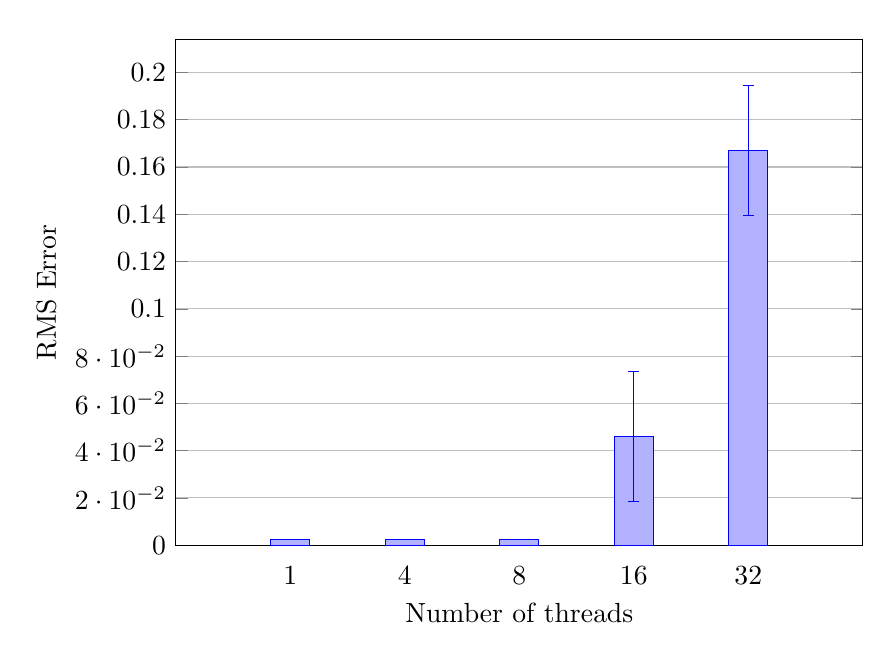
\begin{tikzpicture}
    \begin{axis}[
        xtick=data,
        symbolic x coords={1, 4, 8, 16, 32},
        major x tick style = transparent,
        width  = 0.85*\textwidth,
        height = 8cm,
        major x tick style = transparent,
        ybar=2*\pgflinewidth,
        bar width=14pt,
        ymajorgrids = true,
        ylabel = {RMS Error},
        xlabel = {Number of threads},
        xtick = data,
        enlarge x limits=0.25,
        try min ticks=10,
        ymin=0,
        legend cell align=left,
		legend style={
	        anchor=south east,
	        column sep=1ex
	    },
        ]
            \addplot+[error bars/.cd,
                       y dir=both, y explicit]
                    coordinates {
                    (1, .002544)  +- (0, 0)
                    (4, .002544)  +- (.000000027, .000000027)
                    (8, .002544)  +- (.0000000269, .0000000269)
                    (16, .046)  +- (.0274, .0274)
                    (32, .167)  +- (.0274, .0274)
                    };
\end{axis}
\end{tikzpicture}
	\caption[Error as related to number of threads.]{Error results for a varying number of threads in non-SIMD mode. These
tests were done on computer B, using the $\sin(x)$ potential with a grid size of 300 by 300. The error appears to be roughly proportional to the number of threads one the number of cores on the processor are saturated.}
\label{fig:err-numthreads}
\end{figure}

